% This LaTeX document needs to be compiled with XeLaTeX.
\documentclass[
  10
]{article}
\usepackage[margin=2cm,includehead=true,includefoot=true,centering,]{geometry}
\usepackage{xcolor}
\usepackage{ucharclasses}
\usepackage{hyperref}
\usepackage{amsmath,amssymb}
\usepackage{amsfonts}
\usepackage[version=4]{mhchem}
\usepackage{stmaryrd}
\usepackage{bbold}
\usepackage{polyglossia}
\usepackage{fontspec}
\usepackage{ctex}
\usepackage[export]{adjustbox}
\usepackage{tabularx}
\usepackage{booktabs}

\usepackage{setspace}
\setstretch{1.2}

\makeatletter
\@ifundefined{KOMAClassName}{% if non-KOMA class
  \IfFileExists{parskip.sty}{%
    \usepackage{parskip}
  }{% else
    \setlength{\parindent}{0pt}
    \setlength{\parskip}{6pt plus 2pt minus 1pt}}
}{% if KOMA class
  \KOMAoptions{parskip=half}}
\makeatother
\usepackage{longtable,booktabs,array}
\newcounter{none} % for unnumbered tables
\usepackage{multirow}
\usepackage{calc} % for calculating minipage widths
% Correct order of tables after \paragraph or \subparagraph
\usepackage{etoolbox}
\makeatletter
\patchcmd\longtable{\par}{\if@noskipsec\mbox{}\fi\par}{}{}
\makeatother
% Allow footnotes in longtable head/foot
\IfFileExists{footnotehyper.sty}{\usepackage{footnotehyper}}{\usepackage{footnote}}
\makesavenoteenv{longtable}
\usepackage{graphicx}
\makeatletter
\newsavebox\pandoc@box
\newcommand*\pandocbounded[1]{% scales image to fit in text height/width
  \sbox\pandoc@box{#1}%
  \Gscale@div\@tempa{\textheight}{\dimexpr\ht\pandoc@box+\dp\pandoc@box\relax}%
  \Gscale@div\@tempb{\linewidth}{\wd\pandoc@box}%
  \ifdim\@tempb\p@<\@tempa\p@\let\@tempa\@tempb\fi% select the smaller of both
  \ifdim\@tempa\p@<\p@\scalebox{\@tempa}{\usebox\pandoc@box}%
  \else\usebox{\pandoc@box}%
  \fi%
}
% Set default figure placement to htbp
\def\fps@figure{htbp}
\makeatother
\setlength{\emergencystretch}{3em} % prevent overfull lines
\providecommand{\tightlist}{%
  \setlength{\itemsep}{0pt}\setlength{\parskip}{0pt}}


\hypersetup{colorlinks=true, linkcolor=blue, filecolor=magenta, urlcolor=cyan,}
\urlstyle{same}

\usepackage{colortbl}
\definecolor{table-row-color}{HTML}{999999}
\definecolor{table-rule-color}{HTML}{999999}
%\arrayrulecolor{black!40}
\arrayrulecolor{table-rule-color}     % color of \toprule, \midrule, \bottomrule
\setlength{\aboverulesep}{0pt}
\setlength{\belowrulesep}{0pt}


\setotherlanguages{english}
\IfFontExistsTF{Source Han Serif CN}
{\newfontfamily\chinesefont{Source Han Serif CN}}
{\IfFontExistsTF{Noto Serif CJK SC}
  {\newfontfamily\chinesefont{Noto Serif CJK SC}}
  {\IfFontExistsTF{SimSun}
    {\newfontfamily\chinesefont{SimSun}}
    {\IfFontExistsTF{FangSong}
      {\newfontfamily\chinesefont{FangSong}}
      {\newfontfamily\chinesefont{Arial Unicode MS}}
}}}
\IfFontExistsTF{Times New Roman}
{\newfontfamily\englishfont{Times New Roman}}
{\IfFontExistsTF{Liberation Serif}
  {\newfontfamily\englishfont{Liberation Serif}}
  {\IfFontExistsTF{DejaVu Serif}
    {\newfontfamily\englishfont{DejaVu Serif}}
    {\newfontfamily\englishfont{Arial}}
}}


\author{}
\date{}

\begin{document}


\section{第十七届（2024年）}\label{ux7b2cux5341ux4e03ux5c4a2024ux5e74}

\section{北京市大学生物理实验竞赛}\label{ux5317ux4eacux5e02ux5927ux5b66ux751fux7269ux7406ux5b9eux9a8cux7adeux8d5b}

\section{参赛项目说明书}\label{ux53c2ux8d5bux9879ux76eeux8bf4ux660eux4e66}

参赛题目 ：（请画选择）

题目一：光纤√

题目二：微弱磁场测量

题目三：实验制作（ 定量类 演示类）

题目四：论文（ 教学型 科研型）

北京市大学生物理实验竞赛组委会制

2024 年 3 月

\subsection{实验概述}\label{ux5b9eux9a8cux6982ux8ff0}

随着社会老龄化现象的加剧和健康意识的普遍提高，大众对健康监测的需求愈发迫切。近年来，家用监护设备特别是脉搏监护装置迅速发展。然而，现有的临床心电监护仪体积庞大，操作复杂，难以实现便携式在线生理参数监测。而便携式智能手环虽能监测静止、睡眠、走路等稳定状态下的心率，但是在人体剧烈运动后大量出汗时，由于汗液对光的吸收散射等原因，会产生较大的测量误差。

针对以上问题，本项目基于锥形无芯光纤（Taperednocore
fiber,TNCF）对微弱振动敏感的特性，研制单模-锥形无芯-单模（Singlemode-Tapered
no core-Singlemode,
STNS）光纤结构的传感探头，并应用于人体脉搏在线监测系统。该系统由STNS光纤传感探头、液囊、光源、探测器和Arduino
单片机组成。STNS 光纤传感器的振动灵敏度为
0.21dB/kPa，探测极限为0.286kPa，远低于正常脉压范围，响应时间为
6.230ms，且具备良好的耐久性。采用聚二甲基硅氧烷（PDMS）封装STNS传感探头，并将其密封在液囊中，有效消除了传感探头与脉搏位置精确对准的问题，实现了人体脉搏的实时监测。并通过采集大量的数据，利用随机森林算法预测收缩压（SystolicBlood
Pressure, SBP）和舒张压（Diastolic Blood Pressure,
DBP），其中收缩压的平均偏差（Mean）和误差标准差（SD）为 0.41± 1.98
mmHg，舒张压的平均偏差和误差标准差为
\(\mathbf { 0 . 0 8 \pm 1 . 4 4 ~ m m H g }\)
，符合美国医疗仪器促进协会（AAMI）的血压计认证标准规定。由此可知，本项目提出的传感系统实现了人体脉搏、心率和血压的精确、稳定和实时监测，在心血管健康监测方面具有巨大的潜力。

\subsection{一、设计原理}\label{ux4e00ux8bbeux8ba1ux539fux7406}

\subsection{1.1
基于无芯光纤损耗特性的脉搏测量原理}\label{ux57faux4e8eux65e0ux82afux5149ux7ea4ux635fux8017ux7279ux6027ux7684ux8109ux640fux6d4bux91cfux539fux7406}

对于无芯光纤而言，周围环境即为包层，因此无芯光纤对外界环境的变化非常敏感。根据光纤光学，光纤微弯的总损失功率
\(. a ( t )\) 为{[}1{]}：

\[
\alpha (t) = 6 4 m D ^ {2} (t) \frac {c _ {1} ^ {6}}{c _ {2} ^ {4}} \left(\frac {a ^ {4}}{r ^ {2} \Delta^ {2}}\right)\tag{1}
\]

其中， \(m\) 是光纤上的微弯曲形变的个数， \(D ( t )\)
是随时间变化的微弯振幅； \(c _ { I }\) 和 \(c _ { 2 }\)
为常数，与无芯光纤的材料弹性模量和折射率分布有关；r为无芯光纤的半径，
\(a\) 为单模光纤纤芯半径，Δ是光纤纤芯与包层之间的相对折射率。

无芯光纤拉锥后，半径
r减小，根据(1)式，在其他参数不变的情况下，无芯光纤的半径越小，总损失功率越大，以此增大光纤微弯传感的灵敏度。将血管视为半径随血液流动变化的弹性管道，血管直径的改变导致光纤微弯振幅发生变化，进一步影响光纤微弯的总损失功率。在某一时刻t内血管直径为
\(d ( t )\) ，在 \(t + \varDelta t\) 时刻内血管直径为
\(d ( t { + } \varDelta t )\) ，则光纤微弯的总损失功率为：

\[
\alpha (t) = 6 4 m \left(\frac {d (t + \Delta t) - d (t)}{2}\right) ^ {2} \frac {c _ {1} ^ {6}}{c _ {2} ^ {4}} \left(\frac {a ^ {4}}{r ^ {2} \Delta^ {2}}\right)\tag{2}
\]

Powalowshi 提出的人体血压-血管横截面积模型中指出人体动脉血压变化值
\(p ( t )\) 和人体血管横截面积 \(A ( t )\) 变化关系如下{[}2{]}：

\[
p (t) = p _ {d} e ^ {\alpha \left(\frac {A (t)}{A (d)} - 1\right)}\tag{3}
\]

其中， \(p _ { d }\) 为舒张压， \(A ( t )\) 为血管的横截面积，
\(A ( d )\) 为舒张压对应血管的横截面积， \(\alpha = \gamma A ( d )\)
是常量，表示血管刚度的固定值，其大小与样本人群的性别、年龄、健康状况等因素有关，
\(p ( t )\) 的极大值和极小值即分别对应人体收缩压和舒张压。Powalowshi
确定20 岁左右人群的α值、舒张压以及舒张压对应的血管横截面积为
\(\scriptstyle 1 a = 1 . 6 6 5\)
\(p _ { d } { = } 7 6 ~ \mathrm { m m H g }\)
\(\scriptstyle A ( d ) = 4 . 5 2 \ \mathrm { m m } ^ { 2 }\)
。将上述数值代入公式(3)即可得到：

\[
p (t) = 7 6 e ^ {1. 6 6 5 \left(\frac {A (t)}{4 . 5 2} - 1\right)}\tag{4}
\]

综上，动脉血管中的血液周期性变化导致其对管壁压强 \(p ( t )\)
也发生周期性波动，进而引起弹性血管壁直径 \(d ( t )\)
的变化，导致光纤微弯振幅 \(D ( t )\)
产生波动，从而改变无芯光纤总损失功率 \({ \dot { \alpha } } ( t )\)
。因此，可以通过监测功率变化进而监测脉搏信号变化。

\subsection{1.2
采用液囊优化传感效果的原理}\label{ux91c7ux7528ux6db2ux56caux4f18ux5316ux4f20ux611fux6548ux679cux7684ux539fux7406}

根据帕斯卡原理，不可压缩静态流体中的任何位置受到外部压力的作用时，压强会立即传递到静态流体中的所有其他位置。为防止传感探头与脉搏位置不精确对准引起的失真对实验测量结果产生影响，本实验设计了一种柔软性液囊。密封在液囊中的光纤传感探头能够接收到来自液囊底座的脉搏波信号，从而成功实现了空间不敏感和传感探头与脉搏的自由对准。此外，液囊设计改善了光纤传感器与身体之间的耦合，从而实现更精确的脉搏监测。

\subsection{二、实验方案、步骤及结果分析}\label{ux4e8cux5b9eux9a8cux65b9ux6848ux6b65ux9aa4ux53caux7ed3ux679cux5206ux6790}

\subsection{2.1STNS传感探头的研制及其特性研究}\label{stnsux4f20ux611fux63a2ux5934ux7684ux7814ux5236ux53caux5176ux7279ux6027ux7814ux7a76}

\subsection{1、STNS传感探头的研制}\label{stnsux4f20ux611fux63a2ux5934ux7684ux7814ux5236}

将无芯光纤与单模光纤进行熔接，形成单模-无芯-单模光纤结构传感探头，并固定在拉锥系统的拉伸平台上，将无芯光纤由
\(1 2 5 \mu \mathrm { m }\) 拉至 \(2 7 . 4 \mu \mathrm { m }\) ，如图 1
(a) 所示。将 PDMS 前驱体和固化剂以10：1 的质量比混合均匀，制备 PDMS
薄膜，在薄膜上放置传感探头并均匀涂抹一层 PDMS 溶液，静置后置于
\(8 0 . 0 ^ { \circ } \mathrm { C }\)
的加热平台加热3min，将传感探头密封在PDMS中。传感探头制作流程如图1
(b)所示。

\begin{enumerate}
\def\labelenumi{(\alph{enumi})}
\tightlist
\item
\end{enumerate}

\pandocbounded{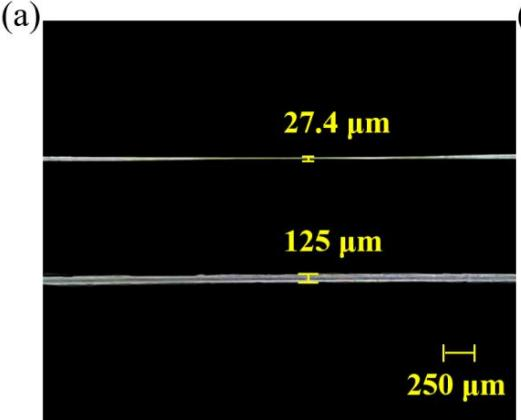
\includegraphics[keepaspectratio,alt={image}]{images/aec09e8e329a0aca360009c6e8598662cfa86b20c2cf89c47aab35e5df8c97f8.jpg}}

\pandocbounded{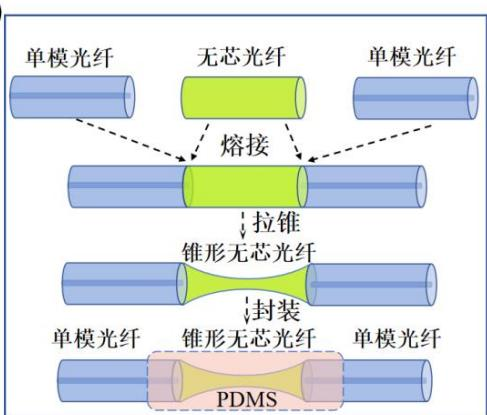
\includegraphics[keepaspectratio,alt={image}]{images/d801f76cbc9655d50c3d64efa61511abc576aef22d3d303b509d138f4c52433e.jpg}}

图 1 (a) 无芯光纤拉锥前后示意图 (b) STNS 传感探头研制示意图

\subsection{2、STNS传感探头的静态响应测试}\label{stnsux4f20ux611fux63a2ux5934ux7684ux9759ux6001ux54cdux5e94ux6d4bux8bd5}

\subsection{（1）实验装置}\label{ux5b9eux9a8cux88c5ux7f6e}

为评估该传感探头的性能，搭建了如图 2 所示的应力传感系统，包括 650nm
激光光源、STNS光纤结构传感探头、光功率计、数字推拉力计以及六维耦合平台。将分辨率为
0.001N、量程为
2N的数字推拉力计（DS2-2N）牢固地安装在支架上，推拉力计探头的面积为
\(1 . 7 6 7 \mathrm { c m } ^ { 2 }\) （如图2的插图所示），STNS
光纤传感探头夹在推拉力计探头和六维耦合平台的右平面之间。通过调整六维耦合平台的微位移旋钮，将应变施加在传感探头上。当探头受到外部应变作用时，锥形光纤发生微弯，光功率产生损耗。为保证传感探头能够实现心率和血压的精确监测，对传感探头的静态参数进行分析，

包括测量其灵敏度、可逆性和探测极限等参数。

\pandocbounded{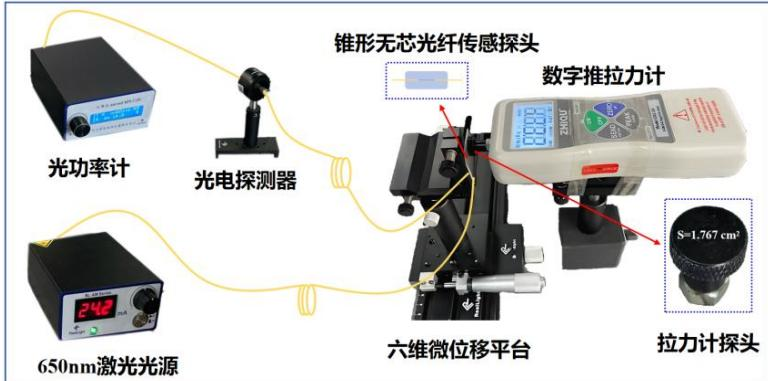
\includegraphics[keepaspectratio,alt={image}]{images/ee39787fc4a1e56be7e3eedc8b8968f07f1e29559201d3021fe448f773619611.jpg}}

图 2 静态参数测量实验装置示意图

\subsection{（2）数据测量与分析}\label{ux6570ux636eux6d4bux91cfux4e0eux5206ux6790}

选择测量范围为 0\textasciitilde1N，步长为
0.005N，记录压力变化过程中输出功率的变化，将压力和输出功率分别换算为压强和损耗，并对数据进行了拟合，结果如图3
(a) 所示。传感器的灵敏度约为 0.21dB/kPa，线性度为
0.9926。为了评估传感器的可逆性，将应力以0.005N为步长从0N变化到1N，再从
1N变化到0N，分别记录每个应力下的输出功率，将应力和输出功率分别换算为压强和损耗，实验结果如图
3(b)
所示。可以看出，在压强增减的过程中，损耗的波动很小，最大波动约为0.04dB（对应压强波动为0.19kPa）。由此可知，该传感器具有很好的可逆性。由于光源和外界环境的影响，输出功率会在一定范围内波动。传感探头在
\(\mathrm { P } { = } 1 . 7 2 \ \mathrm { k P a }\) 和
\(\mathrm { P } { = } 2 . 5 5 \mathrm { k P a }\)
的固定压强下，保证其他条件都不变，每隔 30
秒读取并记录功率数值，其结果如图 3(c)
所示，得到传感探头的损耗波动范围约为0.06dB。计算结果表明，传感探头探测极限为
0.286kPa，而人体正常脉压（收缩压和舒张压的差值）变化范围为30\textasciitilde40mmHg，即
3.99\textasciitilde5.32
kPa。由此得出传感探头的探测极限远小于正常脉压变化范围。这意味着传感器能够精确检测到细微的脉搏波动，确保在实际应用中能够实现高精度的脉搏监测，有效满足健康监测需求。

\pandocbounded{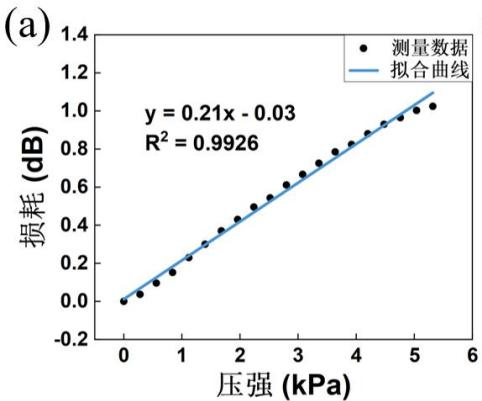
\includegraphics[keepaspectratio,alt={image}]{images/d5f7f9a666f22c0be48652b80b2aedb0a0599da704404e9eed278e2417bfba60.jpg}}

\pandocbounded{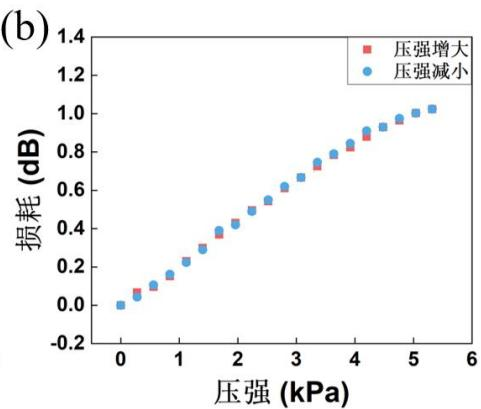
\includegraphics[keepaspectratio,alt={image}]{images/83fde434c25818abe902687fc7a58a21d3d1714e460911469adb4188b0c29d52.jpg}}

\pandocbounded{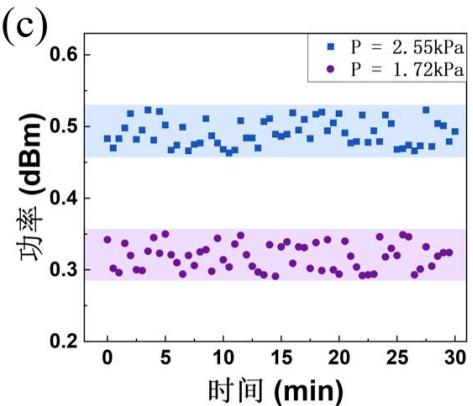
\includegraphics[keepaspectratio,alt={image}]{images/7c75249f662f4d6f7223da2ea5ce758394c5331e8c9efc9adfdd9591f18635b8.jpg}}

图 3 (a) 不同压强下的损耗值和拟合曲线 (b) 可逆性测试结果 (c) 稳定性测试

\subsection{3、STNS传感探头的动态响应测试}\label{stnsux4f20ux611fux63a2ux5934ux7684ux52a8ux6001ux54cdux5e94ux6d4bux8bd5}

为了评估该传感探头在心率和血压实时检测中的应用性能，测量了该传感探头的响应时间。实验中采用自由下落的乒乓球给传感探头施加瞬时应力，模拟真实环境中传感器接收到的信号{[}4{]}。测量结果显示，传感器从强度变化10\%到90\%的响应时间约为6.230
ms，如图 4(a)
所示，响应时间较短，能够满足实时心率和血压检测的需求。为评估本传感探头的耐久性，使STNS光纤传感探头在P=1.72kPa
的固定压强下接受由压电陶瓷产生的 10 Hz
振动信号，通过光电探测器和示波器捕获 100s 的强度变化，最终结果如图 4 (b)
所示。在 1000 个循环中，标准偏差约为 0.41\%，强度基线保持相对稳

定，表明该传感探头具有较好的耐久性。

\pandocbounded{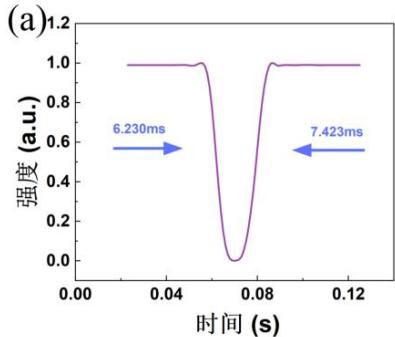
\includegraphics[keepaspectratio,alt={image}]{images/4e1a954acf5a2008542d289b59e5894435c282d9e7465078aac752010d13221b.jpg}}

\pandocbounded{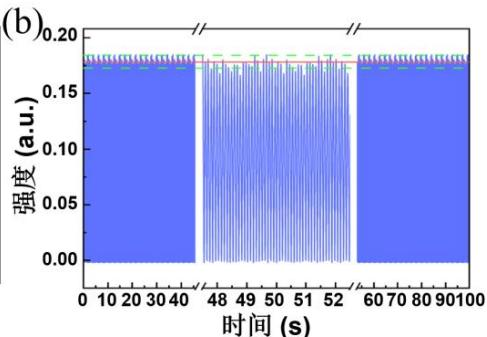
\includegraphics[keepaspectratio,alt={image}]{images/675447f5a86e8d27860cf2849b3f0b285328b565cd8e6243ef4f5ad5586a1941.jpg}}

图 4 (a) 响应时间测试 (b) 耐久性测试

\subsection{2.2 液囊研制}\label{ux6db2ux56caux7814ux5236}

将制备好的PDMS溶液倒入圆形模具中，置于
\(8 0 . 0 ^ { \circ } \mathrm { C }\) 的加热平台上加热10 min，形成23mm
直径、 \(4 0 0 \mu \mathrm { m }\) 厚的圆形 PDMS基底，并将密封在PDMS
薄膜中的STNS传感探头与基底连接，待其凝固后使用注射器将甘油注入基底和薄膜之间，甘油填充区直径23
mm、深度1.5mm，然后用PDMS溶液封住注射口，待 PDMS
完全凝固，密封在液囊中的传感探头制作完成。密封在液囊中的传感探头制作过程以及制作的实物图如图5所示。

\pandocbounded{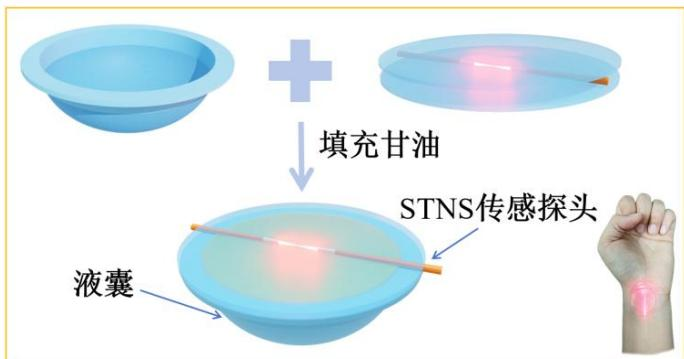
\includegraphics[keepaspectratio,alt={image}]{images/a370927660a96d983024c90d8ab8f9007ffc4fc83f6479a39ca0cc67ee3117cf.jpg}}

图 5 密封在液囊中的传感探头研制过程与实物图

\subsection{2.3
光纤型脉搏测量系统及其应用}\label{ux5149ux7ea4ux578bux8109ux640fux6d4bux91cfux7cfbux7edfux53caux5176ux5e94ux7528}

\subsection{1、脉搏测量系统}\label{ux8109ux640fux6d4bux91cfux7cfbux7edf}

为使脉搏监测系统小型化、便携化，图6(a)
显示了用于精确监测心率和血压的基于STNS传感探头的集成式脉搏测量系统，包括650nm激光光源，STNS
传感探头、光敏二极管、Arduino
单片机和电脑。为了评估该系统的准确性，用商用血压测量仪作校准。光传输到与液囊集成的STNS传感探头中，携带了脉搏信息的输出光信号被光敏二极管检测，将光信号转化为电信号，由Arduino
单片机进行采集并将数据传输到计算机终端，获得实时脉搏波信号，实现心率与血压的测量。实验装置示意图和实物图如图6(a)和(b)
所示。

\begin{enumerate}
\def\labelenumi{(\alph{enumi})}
\tightlist
\item
\end{enumerate}

\pandocbounded{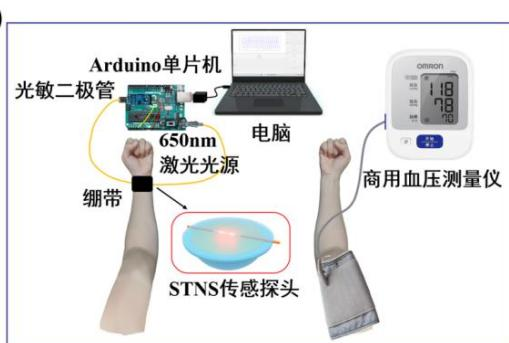
\includegraphics[keepaspectratio,alt={image}]{images/6f2b1e999784a823b9d5d1e80c72508546703d5c2b9e511dc123f8ef0e943c9a.jpg}}

\begin{enumerate}
\def\labelenumi{(\alph{enumi})}
\setcounter{enumi}{1}
\tightlist
\item
\end{enumerate}

\pandocbounded{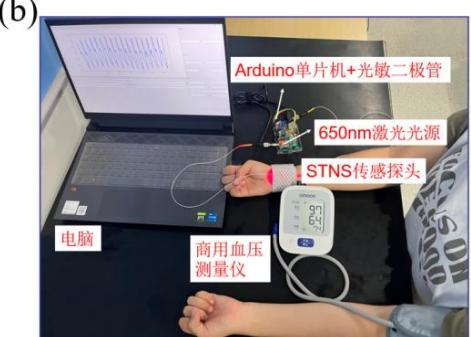
\includegraphics[keepaspectratio,alt={image}]{images/5559d7282c0c86ccf0a7b72215391b66e7dec975779682b831c59f78796669f7.jpg}}

图 6 基于 STNS 传感探头的集成式脉搏测量系统 (a) 实验装置示意图 (b)
实验装置实物图

\subsection{2、脉搏数据测量与分析}\label{ux8109ux640fux6570ux636eux6d4bux91cfux4e0eux5206ux6790}

\subsection{（1）脉搏波形的测量}\label{ux8109ux640fux6ce2ux5f62ux7684ux6d4bux91cf}

将与液囊集成的
STNS传感探头固定在静息状态下的志愿者桡动脉处，脉搏波形显示在电脑上，很清晰地显示出脉搏波的三个典型峰(主波、潮汐波和重搏波)，如图7
(a) 所示。对采集到的15秒脉搏特征信号进行快速傅里叶变换，如图7(b)
所示，可知静息状态下的心率为69bpm (beat
perminute)。对志愿者运动后3分钟内的心率信号进行数据采集，每分钟记录一次，测得结果如图7(c)
所示。从中可以看出，志愿者运动后的心率随着时间的推移而下降，直至恢复到正常状态。运动
1 分钟后心率为
101bpm，脉搏波信号表现出较大的幅值，并且可以观察到潮汐波、重搏波在运动后的某些时期模糊甚至消失。运动
3分钟后心率为69bpm，接近静息时的状态，脉搏波形清晰可见。

\pandocbounded{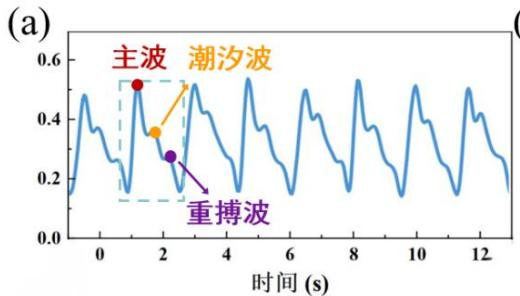
\includegraphics[keepaspectratio,alt={image}]{images/ba00774bb6f93aaec8703e18c1047384ea58f24f24ce33f25aa1b4c656b55e1f.jpg}}

\pandocbounded{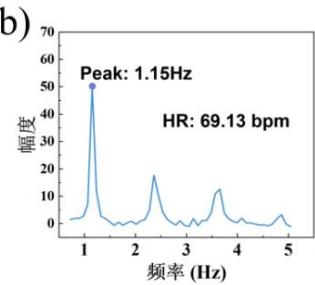
\includegraphics[keepaspectratio,alt={image}]{images/5ba65f3299bef8ecb29d0c531e6cde117f729b7793017694a73186bd9c65bb44.jpg}}

\pandocbounded{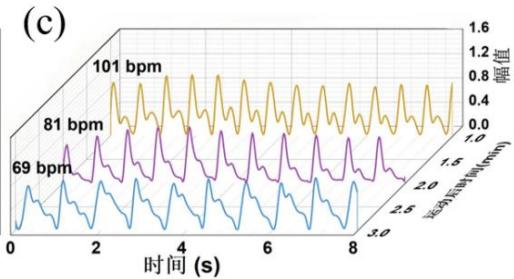
\includegraphics[keepaspectratio,alt={image}]{images/7a2b4099aff0ef47fe65b29b3184d3da446f1618a9f1be2af37023f0d2a072f5.jpg}}

图 7 (a) 电脑显示的脉搏波形图 (b) 频域下的脉搏波形图 (c) 运动后
3分钟内脉搏波形图

为验证液囊的有效性，在桡动脉区域绘制了一个面积为
\(1 5 { \times } 1 5 \ \mathrm { m m } ^ { 2 }\) 的 16 点网格，如图 8
(a)
所示。将液囊中心放置在网格中不同位置以获取脉冲信号，测量的脉搏波形图及其相应的传感探头位置如图8
(b) 所示。测量结果表明，当传感探头放置于
\(1 5 { \times } 1 5 \mathrm { m m } ^ { 2 }\) 的16
点网格中，可成功检测到高保真脉冲信号，成功地消除了位置漂移和错位。

\begin{enumerate}
\def\labelenumi{(\alph{enumi})}
\tightlist
\item
\end{enumerate}

\pandocbounded{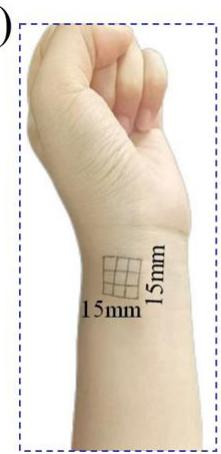
\includegraphics[keepaspectratio,alt={image}]{images/85ea976f8f4797780d34e95117f839dc6521d94b28d09665efb472d219d11bae.jpg}}

\pandocbounded{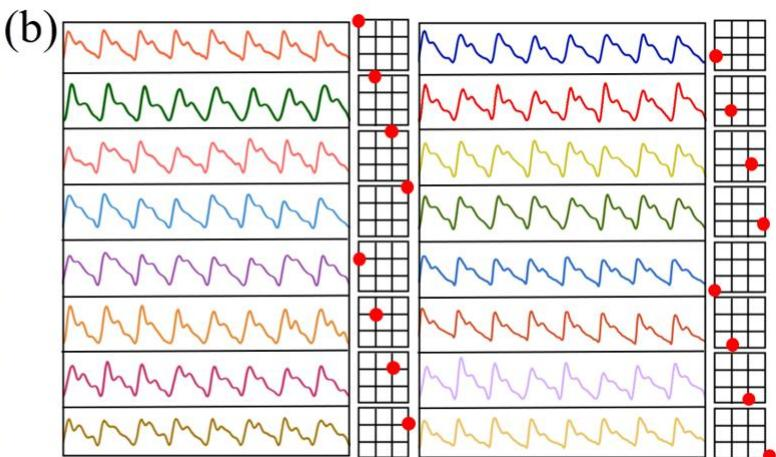
\includegraphics[keepaspectratio,alt={image}]{images/54f7c4ee7868ab77e24227d36fd03c6f17c6130e1bebdcea66085c6aef41a9b9.jpg}}

图 8 (a) 手腕 \(1 5 \times 1 5 \mathsf { m m } ^ { 2 }\) 的 16 点网格图
(b) 传感探头在网格不同点对应的位置及脉搏波形图

\subsection{（2）血压的测量}\label{ux8840ux538bux7684ux6d4bux91cf}

在心室搏动过程中，心脏不断收缩和舒张，进而导致主动脉血管壁收缩和扩张，血容量的周期性增加和减少形成了脉搏信号的波状压力变化，其形状、周期、峰值和波形特征等特征与心血管健康水平密切相关。因此，脉搏波信号的特征蕴含着丰富的血压生理和病理信息，具有较高的医学价值{[}4{]}。本项目采用随机森林算法，从测量得到的脉搏波形中选择了10个与血压相关的特征作为输入，用商用血压测量仪（OMRONJ710，心率测量精度为
±5\%，血压测量精度为±
\(3 \ \mathrm { m m H g } \pm 0 . 4 \ \mathrm { k P a } )\)
测量得到的收缩压（SBP）和舒张压（DBP）作为输出，对 20 岁左右的23
名志愿者(13
名男性，10名女性)在不同时间段分别进行了多次数据采集，并记录了 230
组数据，其中
80\%用于模型训练，20\%用于评估和预测。首先对采集到的数据进行预处理，使用截止频率为10
Hz的低通滤波器消除高频干扰带来的噪声。然后通过多项式拟合方法消除由光强度变化和其他扰动引起的基线漂移，提取脉搏波的特征，并构建训练模型来估计血压值。在实验过程中均要求志愿者静坐一段时间后再进行血压测量。将血压测量仪佩戴于距离上臂肘关节10mm
- 20mm处，同时右手腕部佩戴本脉搏监测系统。最终血压预测效果如下：SBP
的平均偏差和误差标准差为 \(0 . 4 1 \pm 1 . 9 8 \mathrm { m m H g }\)
，DBP 的平均偏差和误差标准差为
\(0 . 0 8 \pm 1 . 4 4 \mathrm { m m H g }\)
。美国医疗仪器促进协会（AAMI）的血压计认证标准规定，平均偏差必须小于 5
mmHg，标准偏差必须小于 8 mmHg。因此，本脉搏测量系统满足要求。预测值 SBP
和DBP 的相关系数分别为 0.95 和0.94，如图 9 (a)和(b)
所示，表明本脉搏测量系统与参考血压计具有良好的相关性。此外，SBP 和 DBP
的 Bland - Altman 图如图 9 (c)和(d) 所示，其中 SBP 的平均偏差值为 0.41
mmHg，95\%置信区间
\(( \mathrm { M e a n } \pm 1 . 9 6 \mathrm { S D } )\) ）为-3.46 mmHg
到 4.28 mmHg，DBP 的平均偏差值为 0.08 mmHg，95\%置信区间介于-2.75 mmHg
至 2.91 mmHg 之间，且绝大多数结果均在
95\%的置信区间内，表明本系统测量的血压值准确且与商用血压测量仪一致性较好。

\pandocbounded{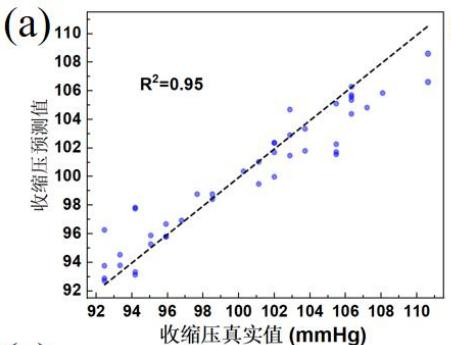
\includegraphics[keepaspectratio,alt={image}]{images/2c6e0436e6249f3ee5695ce60283040599aa48b2e024fbd5c5a0060a650c7fe5.jpg}}

\begin{enumerate}
\def\labelenumi{(\alph{enumi})}
\setcounter{enumi}{1}
\tightlist
\item
\end{enumerate}

\pandocbounded{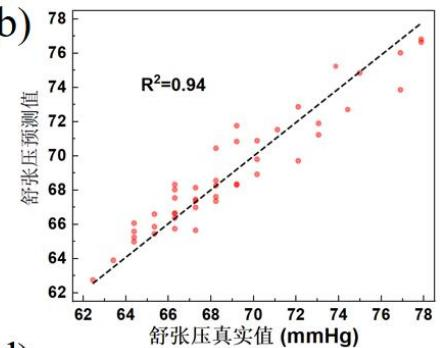
\includegraphics[keepaspectratio,alt={image}]{images/ffe1c316d9607e0aee79d1b9dd266d62f8cdf1a34347896ece958b1aeabc0f95.jpg}}

\begin{enumerate}
\def\labelenumi{(\alph{enumi})}
\setcounter{enumi}{2}
\tightlist
\item
\end{enumerate}

\pandocbounded{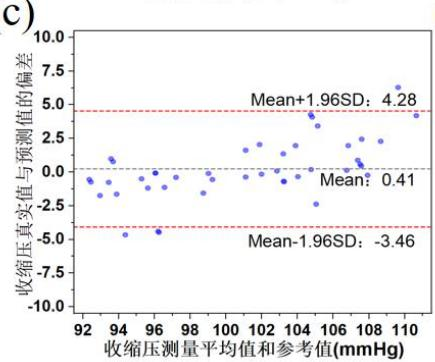
\includegraphics[keepaspectratio,alt={image}]{images/a828c603110f0a92e8e5d57aad9381c15801d9fe2379fec9a0e5914e7a78dd55.jpg}}

\begin{enumerate}
\def\labelenumi{(\alph{enumi})}
\setcounter{enumi}{3}
\tightlist
\item
\end{enumerate}

\pandocbounded{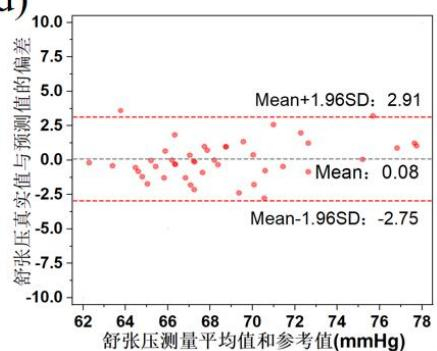
\includegraphics[keepaspectratio,alt={image}]{images/3e416a552f7119affa5029bc14f83ed265b5dc85a2472e1ac4bba48080152c44.jpg}}

图 9 (a) SBP 相关性分析 (b) DBP 相关性分析 (c) SBP 的 Bland-Altman 图
(d) DBP 的 Bland-Altman 图

\subsection{三、实验数据及误差分析}\label{ux4e09ux5b9eux9a8cux6570ux636eux53caux8befux5deeux5206ux6790}

\subsection{1、实验数据}\label{ux5b9eux9a8cux6570ux636e}

采用本项目研制的脉博测量系统与商用血压测量仪对10位志愿者运动前后的脉搏进行检测，心率结果如表1
所示，静息状态下的血压结果如表2 所示。

表 1 心率测量值及误差

{\def\LTcaptype{none} % do not increment counter
\begin{longtable}[]{@{}lllllll@{}}
\toprule\noalign{}
\endhead
\bottomrule\noalign{}
\endlastfoot
\multirow{2}{*}{} & \multicolumn{3}{l}{%
静息时心率} & \multicolumn{3}{l@{}}{%
运动后心率} \\
& 商用血压仪测量心率值(bpm) & STNS传感探头测量心率值(bpm) & 误差 &
商用血压仪测量心率值(bpm) & STNS传感探头测量心率值(bpm) & 误差 \\
志愿者1 & 84 & 83.94 & 0.07\% & 123 & 122.18 & 0.67\% \\
志愿者2 & 68 & 68.56 & 0.82\% & 93 & 94.51 & 1.62\% \\
志愿者3 & 89 & 88.88 & 0.13\% & 129 & 128.42 & 0.45\% \\
志愿者4 & 69 & 68.63 & 0.54\% & 119 & 118.67 & 0.28\% \\
志愿者5 & 79 & 79.15 & 0.19\% & 121 & 120.27 & 0.60\% \\
志愿者6 & 84 & 83.91 & 0.11\% & 103 & 103.69 & 0.67\% \\
志愿者7 & 82 & 82.74 & 0.90\% & 117 & 117.86 & 0.74\% \\
志愿者8 & 80 & 79.23 & 0.96\% & 124 & 123.27 & 0.59\% \\
志愿者9 & 79 & 79.01 & 0.01\% & 116 & 115.08 & 0.79\% \\
志愿者10 & 79 & 79.02 & 0.02\% & 119 & 118.64 & 0.30\% \\
\end{longtable}
}

表 2 血压测量值及误差

{\def\LTcaptype{none} % do not increment counter
\begin{longtable}[]{@{}lllllll@{}}
\toprule\noalign{}
\endhead
\bottomrule\noalign{}
\endlastfoot
\multirow{2}{*}{} & \multicolumn{6}{l@{}}{%
血压} \\
& 商用血压仪测量收缩压(mmHg) & STNS传感探头测量收缩压(mmHg) & 误差 &
商用血压仪测量舒张压(mmHg) & STNS传感探头测量舒张压(mmHg) & 误差 \\
志愿者1 & 109 & 107.65 & 1.24\% & 65 & 66.27 & 1.95\% \\
志愿者2 & 113 & 110.23 & 2.45\% & 68 & 69.00 & 1.45\% \\
志愿者3 & 101 & 100.14 & 0.85\% & 69 & 68.59 & 0.59\% \\
志愿者4 & 99 & 97.63 & 1.38\% & 62 & 62.34 & 0.55\% \\
志愿者5 & 106 & 104.95 & 0.99\% & 71 & 73.28 & 3.21\% \\
志愿者6 & 102 & 99.76 & 2.20\% & 65 & 66.20 & 1.85\% \\
志愿者7 & 96 & 95.05 & 0.99\% & 62 & 63.04 & 1.68\% \\
志愿者8 & 100 & 98.58 & 1.42\% & 66 & 66.43 & 0.65\% \\
志愿者9 & 107 & 105.82 & 1.10\% & 72 & 71.00 & 1.39\% \\
志愿者10 & 99 & 97.30 & 1.72\% & 70 & 72.08 & 2.97\% \\
\end{longtable}
}

\subsection{五、项目创新与特色}\label{ux4e94ux9879ux76eeux521bux65b0ux4e0eux7279ux8272}

（1）锥形无芯光纤的优势：无芯光纤由于没有包层，对外界环境变化异常敏感，将其通过拉锥的方式减小直径后，变成柔韧性更好、灵敏度更高的微纳光纤。该传感探头灵敏度高达0.21
dB/kPa，能够精确捕捉细微的脉搏跳动，远高于传统的光电容积脉搏波描记法的灵敏度。

（2）液囊的优势：液囊的使用有效消除了传感器在桡动脉区域的位置漂移和错位问题，提高了脉搏信号捕获的准确性，使得在桡动脉
\(1 5 \times 1 5 \mathrm { m m } ^ { 2 }\)
的网格不同点位上获取的脉搏波形图具有高度可靠性与保真度。

（3）集成与小型化设计：利用光敏二极管和 Arduino
单片机，将光功率信号转换为电信号变化发送到电脑，实现实时显示心率、血压、脉搏波形图等功能，完成系统集成化和小型化。

（4）随机森林预测血压：结合随机森林抗过拟合、抗噪声和处理复杂数据结构等优势，训练和验证大量脉搏特征数据，实现了对收缩压和舒张压的高精度预测。其中
SBP 的平均偏差和误差标准差为 0.41 ± 1.98 mmHg，DBP
的平均偏差和误差标准差为 0.08 ± 1.44 mmHg，符合 AAMI
血压计认证标准规定，有望用于人体健康穿戴设备。

\subsection{六、制作成本}\label{ux516dux5236ux4f5cux6210ux672c}

{\def\LTcaptype{none} % do not increment counter
\begin{longtable}[]{@{}|l|l|l|l|@{}}
\toprule\noalign{}
\endhead
\bottomrule\noalign{}
\endlastfoot
\hline
名称 & 单价（元） & 数量 & 金额（元） \\
\hline
2m单模光纤 & 6 & 1 & 6 \\
\hline
1m无芯光纤 & 50 & 1 & 50 \\
\hline
650nm激光光源 & 72 & 1 & 72 \\
\hline
光敏二极管 & 2 & 1 & 2 \\
\hline
Arduino单片机 & 64 & 1 & 64 \\
\hline
总价 & \multicolumn{3}{l@{}}{%
194元} \\
\hline
\end{longtable}
}

\subsection{参考文献}\label{ux53c2ux8003ux6587ux732e}

{[}1{]}
冉艳丽.可调谐光纤激光器及其传感应用研究{[}D{]}.湖北:华中科技大学,2016.

{[}2{]}
谭胜.面向动脉血压检测的柔性超声波微传感器研究{[}D{]}.哈尔滨工业大学,2021.

{[}3{]} 李孟强.基于锥形光纤的高照度 LED
光源的聚光特性研究{[}D{]}.燕山大学,2022.

{[}4{]} LI L, SHENG S, LIU Y, et al.~Automatic and continuous blood
pressure monitoring via an optical-fiber-sensor-assisted
smartwatch{[}J/OL{]}. PhotoniX, 2023, 4(1): 21.

注意：

竞赛采用匿名评审，说明书里不允许出现任何参赛队和参赛学校信息。

邮箱: wlsyzx@bjtu.edu.cn 联系电话: 51683629，13811861683 贺敬文

通信地址：北京交通大学物理国家级实验教学示范中心 邮编:100044

\end{document}
